\documentclass[12 pt]{article}
\usepackage{hyperref}
\usepackage{fancyhdr}
\usepackage{setspace}
\usepackage{enumerate}
\usepackage{amsmath}
\usepackage{lastpage}
\usepackage{mathtools,float}
\usepackage{tikz}
\usepackage{tabularx}
\usepackage{ltablex}
\usepackage{amssymb}
\usepackage{textcomp}
\usepackage[T1]{fontenc}
\usepackage{listings}
\usepackage[margin=1 in]{geometry}
\allowdisplaybreaks
%\usepackage[dvipsnames]{xcolor}   %May be necessary if you want to color links
\hypersetup{
	%colorlinks=true, %set true if you want colored links
	linktoc=all,     %set to all if you want both sections and subsections linked
	linkcolor=black,  %choose some color if you want links to stand out
}
\usepackage{graphicx}
\graphicspath{{Images/}}
\author{Julian Lore}
\date{Last updated: \today}
\title{COMP 206: Intro to Software Systems Review}
\pagestyle{fancy}
\lhead{COMP 206}
\chead{\leftmark}
\rhead{Julian Lore}
\cfoot{Page \thepage \ of \pageref{LastPage}}
\newcommand{\tab}[1]{\hspace{.2\textwidth}\rlap{#1}}
\begin{document}
	\onehalfspacing
	\maketitle
	Adapted from Joseph Vybihal's Winter 2017 COMP206 slides.
	\tableofcontents
	\section{Software Systems}
	\subsection{What is a Software System?} 
	A \textbf{system} has several parts. By themselves, not special. They cooperate together to make something. Addition of several sub-systems (programs that depend on other programs). System is the complete application that interacts directly with user.
	\\
	A \href{https://en.wikipedia.org/wiki/Software_system}{software system} consists of a system with components (based on software) that form a part of a computer system. I.e. has separate programs, config files, documentation. Single components from a software system are usually useless without each other.
	\\ In this class, our programs will send instructions to the operating system, which will deal with sending stuff to the actual hardware.
	\subsection{Examples of Software Systems}
	\paragraph{Email} Email clients don't know how to send email, they just send data through a wire. Keeps sending it to the next person (connected in network), until finally ISP or something else knows what to do with the email. Each piece only knows so much, all have to be together to work. 
	\paragraph{Facebook}
	Needs Internet, ISP, PC/phone/browser and then the server/application/database. With only one thing, wouldn't be able to use Facebook.
	\paragraph{Object oriented programming/Java} Requires JVM, computer, etc. Text file $\to$ byte code converter $\to$ JVM $\to$ Libs $\to$ OS $\to$ PC $\to$GPU or Network$\to$Internet
	\paragraph{Internet} The Internet is the quintessential software system! Has many sub-systems, such as:
	\begin{itemize}
		\item Local PC
		\item Server
		\item Network
		\item Encryption
		\item etc.
	\end{itemize} See 1.4 For more information.
	\subsection{Operating Systems}
	\paragraph{Drivers} Small pieces of software, allow external devices to communicate with PC generically. So application does not have to deal separately with all different types of hardware.
	\paragraph{What is an Operating System?} Piece of software, allows users to use computer without knowing inner workings. Main use is to manage resources, execute programs properly. Middle man between low-level hardware \& users/programs. Also provides libraries.
	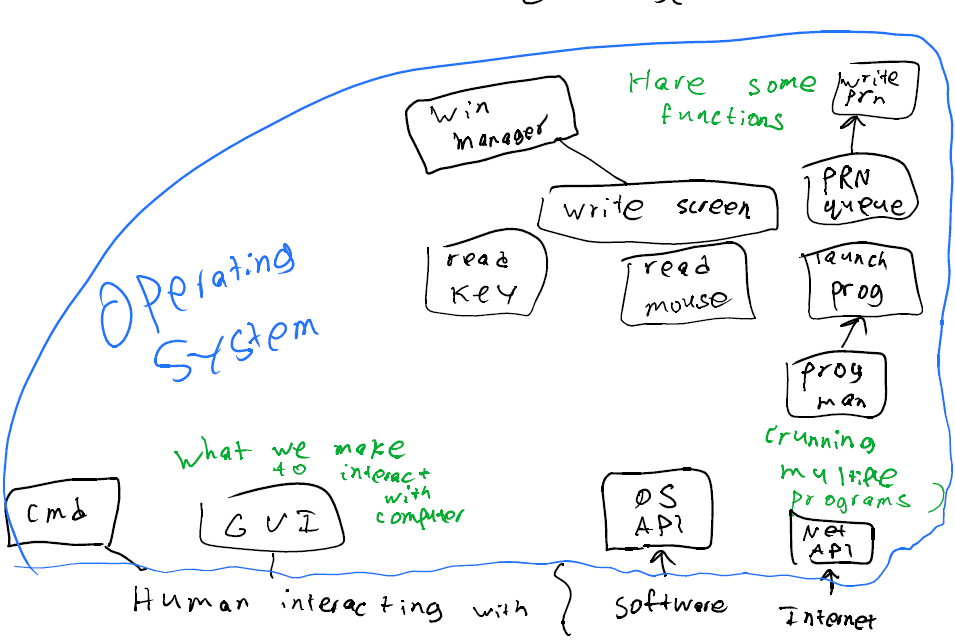
\includegraphics[scale=0.5]{os}
	\paragraph{OS Architecture}
	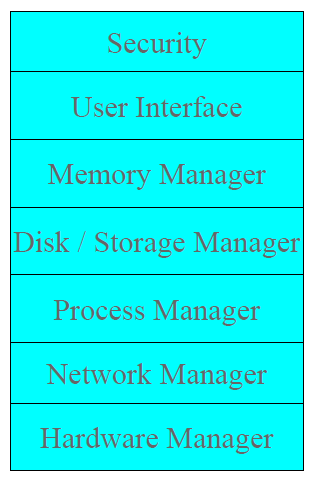
\includegraphics[scale=0.5]{oss} Uses ideas from systems and subsystems.
	\begin{itemize}
		\item Security 
		\begin{itemize}
			\item Passwords
			\item Encryption
			\item File permissions
		\end{itemize}
		\item User Interface
		\begin{itemize}
			\item GUI, CLI, Shell memory
		\end{itemize}
		\item Memory Manager
		\begin{itemize}
			\item Find memory for programs
			\item Format RAM
			\item Manage cache, buffers, spools
		\end{itemize}
		\item Storage Manager
		\begin{itemize}
			\item Secondary Storage
			\item Floppy disks
			\item Hard disks
			\item Memory sticks
			\item etc.
		\end{itemize}
		\item Process Manager
		\begin{itemize}
			\item Runs programs
			\item Multi-processing/multi-CPU
			\item Kills programs
			\item Run-time errors
		\end{itemize}
		\item Network Manager
		\begin{itemize}
			\item LAN
			\item Internet
			\item etc.
		\end{itemize}
		\item Hardware Manager
		\begin{itemize}
			\item Drivers
			\item Assembler \& registers
			\item etc.
		\end{itemize}
	\end{itemize}
	\subsection{Internet} All interconnected computers around the world. 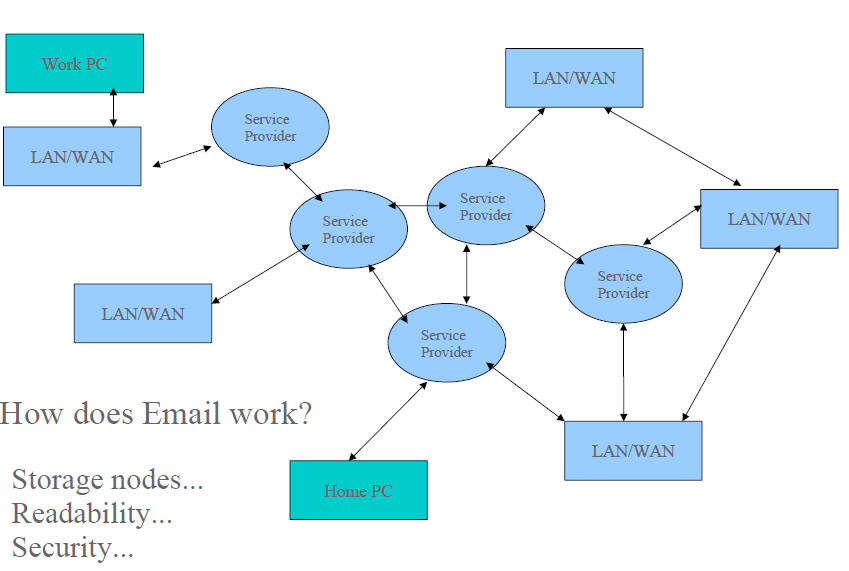
\includegraphics[scale=0.5]{inter}
	\subparagraph{What is a Network?}
	Wire, permits communication between computers. \textbf{LAN:} Local Area Network, computers in same room/building. \textbf{WAN:} Wide Area Network, computers in different buildings/cities, more than 1 server interconnecting big network nodes.
	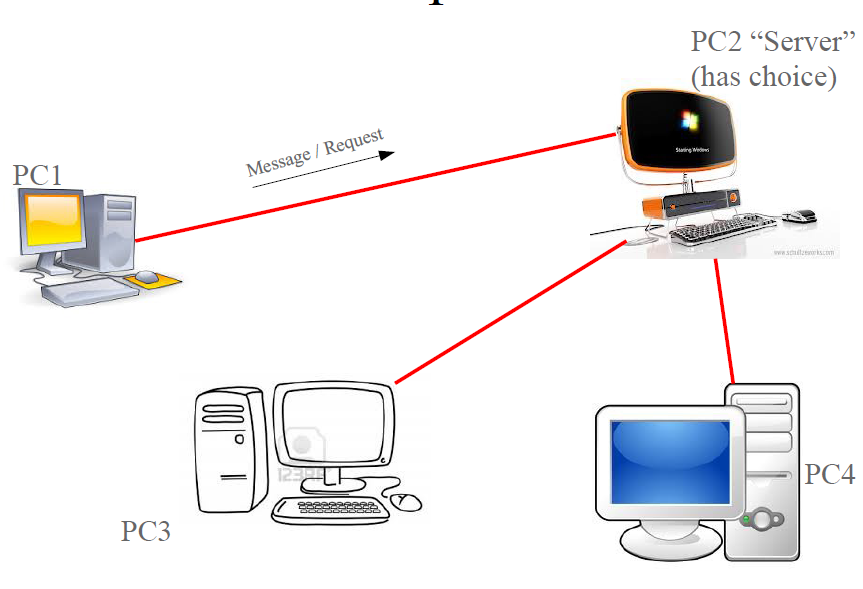
\includegraphics[scale=0.4]{ntw}
	\paragraph{Client/Server}
	\begin{itemize}
		\item Client sends request packet to server
		\item Server tries to find requested thing
		\item Server sends reply packet with data/program
		\item Client copies into memory and executes
	\end{itemize}
	Programs run on client, but programs stored on server, data is spread out. \textbf{MasterComputer/Main frame} is the opposite, programs stored \& run on server, client just sees it.
	Additional terms: \textbf{Handshaking} consists of agreeing on packet format \& passwords. \textbf{Comm-error}, packet lost, resend request or time-out. 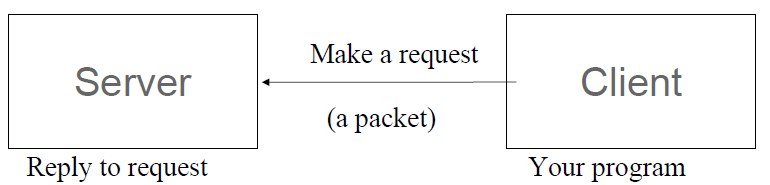
\includegraphics[scale=0.3]{cs}
	\paragraph{Service Providers} Special server, knows locations of other servers on the Internet. Uses this knowledge to deliver package to right destination. Internet = WAN of service providers that are connected to independent LAN \& WAN networks.
	\paragraph{Web} Subset of Internet with only interconnected ISP servers. Interacts solely with browsers.
	\paragraph{Public\_HTML} Servers connected to Internet have a directory/folder called public\_html, which is public. By default, only this is accessible from Browser. The default operation for the Internet is to display folders and files at that Internet address (like a file-browser), like \href{https://www.kernel.org/pub/software/scm/git/}{this}. Need an index.html or other stuff to change default behavior and display a ``web page".
	\paragraph{Communicating with Other Computers} Each computer needs a unique ID, today we use our \textbf{IP Address} as our unique ID number. 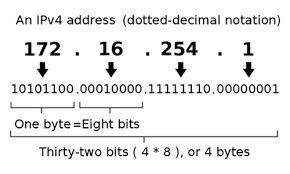
\includegraphics{ipv4}
	\section{Unix}
	\subsection{About Unix}
	\paragraph{History}
	Failed OS by AT\&T Bell Laboratories called Multics, $1^{st}$ OS with 2 windows \& 2 programs at the same time. Ken Thompson was working on project, writing game called \textit{Space Travel}. Ported game to PDP-7 when project was canceled. Wrote Unix to make it easier to port. 3 types: System V UNIX (based off original), BSD UNIX (based on Berkeley Software Distribution) and UNIX-like (behave like UNIX, includes \textbf{Linux}, which we'll be using).
	\paragraph{General Info} Unix is:
	\begin{itemize}
		\item Optimized/simple
		\item Password-based security
		\item Driven by command line
		\item Client-server
		\end{itemize}
		Unix is client/server! Companies buy one huge machine (server) and many small terminals (client). Can SSH into a SOCS machine at school.
	\paragraph{OS Components} Unix is a modular OS. 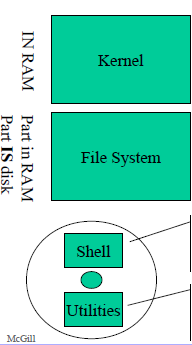
\includegraphics[scale=0.6]{osc} Several components: 
	\begin{itemize}
		\item Kernel
		\begin{itemize}
			\item In RAM
			\item Handles logging in
			\item Task switching
			\item Manages everything
			\item Basic interface
			\item Drivers, run-time stack
		\end{itemize}
		\item File System
		\begin{itemize}
			\item How is disk drive formatted
			\item FAT (File Allocation Table)
			\item Data structure making files "real"
			\item Everything is a "Program"
			\item R/w to disk \& peripherals
		\end{itemize}
		\item Shell
		\begin{itemize}
			\item More advanced UI
			\item Global memory
			\item Commands to interact with shell
		\end{itemize}
		\item Utilities
		\begin{itemize}
			\item Extra commands and programs
			\item Drivers
		\end{itemize}
		%\textbf{Session} consists of Kernel $\to$ File System $\to$ login until logout
	\end{itemize}
	\paragraph{Users} Need an account on a Unix machine to use it. Consists of a user name and password. User gets a \textbf{home directory} ($\sim$). Accounts are members of at least one group. Groups used for permission purposes. Every Unix machine has a \textbf{root} account, with ALL permissions.
	\paragraph{Passwords} Since all Unix security is based on passwords, important to have a good password. Breach consists of someone else logging in with your password. Shouldn't use dictionary words because there are dictionary attacks. Other attacks include getting to know the user and brute force. Want a mix of upper and lower case, numbers, punctuation.
	\subsection{Sessions} 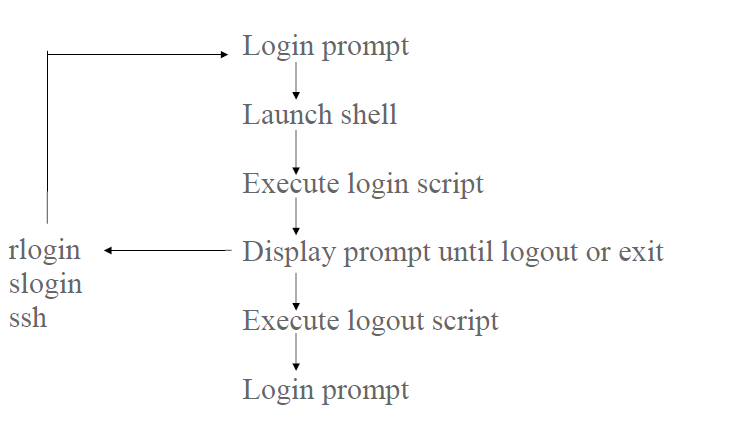
\includegraphics[scale=0.5]{ses} One session goes from login, loops the prompt many times until you logout. rlogin, slogin, ssh used to create another session within a login.
	\paragraph{Environment Session Memory} Has stuff like user name, home, shell, etc.
	\\ When you start the shell, OS sets up environment, a collection of variables which can be accessed from any application launched from that environment. env \& set show you current environment variables. setenv and set are not used in bash to change an environment variable in Bash, just write var=value. Echo can give you specific env variables, like echo \$var.
	\section{Bash/Command-line} 
	\paragraph{Command-line Prompt}Basically a while loop that keeps reading the input you give it until you logout or exit.
	\paragraph{Syntax} Program -switches arguments
	\\ Program is any command or executable. Switches are parameters that modify program's execution, arguments are fed to program. 
	\subsection{Good Commands to Know}
	\begin{tabularx}{\textwidth}{|X|X|X|X|}
		\hline
		Command & Switches/Args & Examples & Usage
		\\\hline
		 ls & -l (long output) & ls ; ls -l ; ls text.txt & lists files and directories
		 \\ & -a (all, hidden) [file/dir] & &
		\\\hline
		 whoami &&& Tells you user logged in as
		 \\\hline
		 who &&& Who is logged on server
		 \\\hline
		 exit &&& exits shell
		 \\\hline 
		 logout &&& logs out of session, can logout of a nested session
		 \\\hline
		 finger & username@host & finger jlore & info on user
		 \\\hline
		 ssh & username@host & ssh jlore@mimi.cs.mcgill.ca & ssh into this user
		 \\\hline
		 mkdir & directoryname & mkdir test & make directory
		 \\\hline 
		 cp & filename destination file & cp a.txt b.txt ; cp a.txt /jl & copy a file
		 \\\hline
		 cd & [directory] [..] & cd test ; cd .. (goes up 1 dir) ; cd (goes home) & change dir
		 \\\hline
		 cat & file & cat test.txt & reads text, concatenates files, can read 2 at once
		 \\\hline
		 rm & file & rm test.txt & removes a file
		 %\\\hline
		 %more & & & paginates text
		 \\\hline
		 sort & -(reverse alphabetical) && sorts text alphabetically
		 \\\hline
		 pwd & && prints working directory
		 \\\hline 
		 rmdir & directory & rm test & removes EMPTY directory
		 \\\hline 
		 chgrp & group file & chgrp friends test.txt & changes group of file
		 \\\hline
		 chmod & u(user)g(group)a(all) & chmod u=r test.txt & change permissions
		 \\ ~&  +(adds perm)-(removes)=(replaces) rwx 421 file &  (changes user to read) &
		 \\ &(0=no perm 1=exec) & chmod 000 test.txt&
		 \\ &(2=write 4=read)& &
		 \\\hline 
		 chown & owner file & chown jlore test.txt & changes owner of file
		 \\\hline
		 mv & file1 file2 & mv test.txt /jlore/test.txt & moves file1 into file2
		 \\\hline 
		 echo & text/string & echo hi & echoes string to stdout
		 \\\hline 
		 head & [-number] file & head -2 test & display first n or first few (if no number) lines of file
		 \\\hline
		 tail & [-number] file & tail -2 test & display last n or last few lines of file
		 \\\hline 
		 more & file & more test & page through file, enter advances a page
		 \\\hline 
		 less & file & less test & navigate through paginated file, better than more
		 \\\hline 
		 man & command/program & man ls & get manual page for a program
		 \\\hline
		 date & [options] & & gets current date \& time
		 \\\hline 
		 du & [options] [dir/file] & du source/ & shows disk space usage
		 \\\hline 
		 hostname &&& Gives name of machine
		 \\\hline 
		 uname & [option] && Prints system info
		 \\\hline 
		 script & file & script record.txt & Records everything appearing on screen (IN/OUT) to file until exit or ctrl-D
		 \\\hline 
		 which & command & which ls & Shows path where command is located
		 \\\hline
		 kill & [options] [-SIGNAL] [pid\#] & kill -9 1234 & Kills a process id, -9 is sigkill, aggressive/forceful kill
		 \\\hline 
		 ps & [options] -a (all processes/users) -e (environment) -g (group leaders too) -l (long) -u (shows user, also more info like \% resources) -x (includes things not run from terms) -f (full)& ps -a & Shows status of active processes
		 \\\hline 
		 top & && Monitors resource usage of active processes
		 \\\hline
		 tar & -c (create new) -r (update) -x (extract) -f (archive name) -v (verbose) -z (compress using gzip) (files/dir)& tar -cvf log.tar *.log ; tar -zcvf log.tgz *.log ; tar -xvf log.tar /tmp/log & Archive manipulation using tar, see 3.2
		 \\\hline
		 diff & [op] file1 file2 & diff text text2 & compares 2 files
		 \\\hline
		 file & [op] file & file text & What ``kind" of file?
		 \\\hline
		 find & [op] [path] expressions & find test & Finds files matching pattern
		 \\\hline
		 ln & -s (soft link) source target & ln fav.txt read & Links source to target. Default is hard link, gives another name to a file. Soft/symbolic link is an indirect pointer, does not affect target file.
		 \\\hline
		 paste & [op] file1 file2 & paste text1 text2 & combines 2 files, one after other
		 \\\hline
		 touch & [op] [date] file & touch text & Create empty file or update access time
		 \\\hline
		 wc & [op] file(s) & wc text & word count
		 \\\hline
		 write & userid & write jlore & Sends text message to someone \textasciicircum D to end, mesg -y/n to turn on/off
		 \\\hline
		 wall &&& write to all
		 \\\hline
		 grep & [op] -i (ignore case) -c (return only count of matches) -v (invert, display ones that don't match) -n (adds line number of match) -l (filenames of matches) string files & grep hi text & Search for occurrences of String, supports regex
		 \\\hline
		 sed & [op] -i (interactive, update current file) files & sed -i \textquotesingle 1d \textquotesingle text (deletes first line) ; sed -i \textquotesingle 1iHello \textquotesingle text (inserts Hello at 1st line) & stream editor
		 \\\hline
		 awk & [op] files & awk \textquotesingle NR==1\textquotesingle text (reads first line) & scan for patterns in file
		 \\\hline
		 clear &&& clears screen/prompt
		 \\\hline
		 expr & math & expr 1 + 2 & Does integer math
		 \\\hline
	\end{tabularx}
	\paragraph{Common switches (mainly cp, mv, rm)}
	\begin{enumerate}[.]
		\item -i: interactive
		\\ prompt and wait for confirmation
		\item -r or -R: recursive
		\\ visits directory recursively, visits files and subdirs
		\item -f: force
		\\ don't prompt for confirmation, overrides -i
	\end{enumerate}
	\paragraph{Killing}
	\textasciicircum Z (ctrl-Z) forceful kill
	\\\textasciicircum C (ctrl-C) gentle kill
	\subsection{Files \& Directories}
	\paragraph{Hidden Files/Folders}: Start with ., i.e. .config \\ Can be seen with ls -a
	\paragraph{Wild cards}
	~\\\begin{tabular}{c|c}
		* & anything
		\\ ? & any single char 
		\\ $[$abc$]$ & a or b or c
	\end{tabular}
	\paragraph{Directories} Directories are folders. Use same permission system as files. Root denoted by /
	\\ Common Unix system has following directories:
	\begin{itemize}
		\item /etc : config files, pws
		\item /bin : OS executables
		\item /usr : Application installations
		\item /opt : Another application installation dir
		\item /dev : Device files for hardware
		\item /var : Files that vary a lot, like logs
	\end{itemize}
	\paragraph{Typical Directory Structure}~\\
	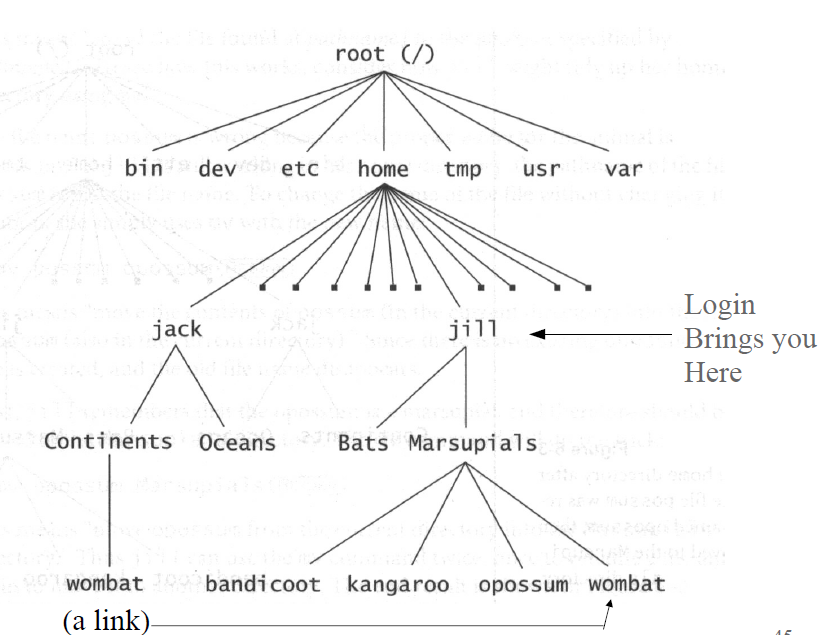
\includegraphics[scale=0.5]{dst}
	\paragraph{Absolute vs Relative Paths}
	\begin{enumerate}[.]
		\item Relative paths: Path from your current directory
		\item Absolute paths: Path from root
		\begin{itemize}
			\item ./folder from current directory, same as folder
			\item ../folder parent directory one up
		\end{itemize}
	\end{enumerate}
	\paragraph{File Descriptors} Created by OS when file opened. Reference to that file. Unix has 3 special file descriptors that are always opened.
	\begin{itemize}
		\item STDIN 0 : keys typed by user gathered here
		\item STDOUT 1 : normal application output sent here
		\item STDERR 2 : where error output is sent
	\end{itemize}
	\paragraph{Permissions}
	Three levels, user, group and other. 3 types of rights, read, write and execute. Can give any combination of these rights to the 3 levels. Permissions usually shown by string of 10 characters, first is if directory or not, then next bunches of 3 are rwx for 3 levels.
		\subparagraph{Directory Listing (ls)}
		Long format: \\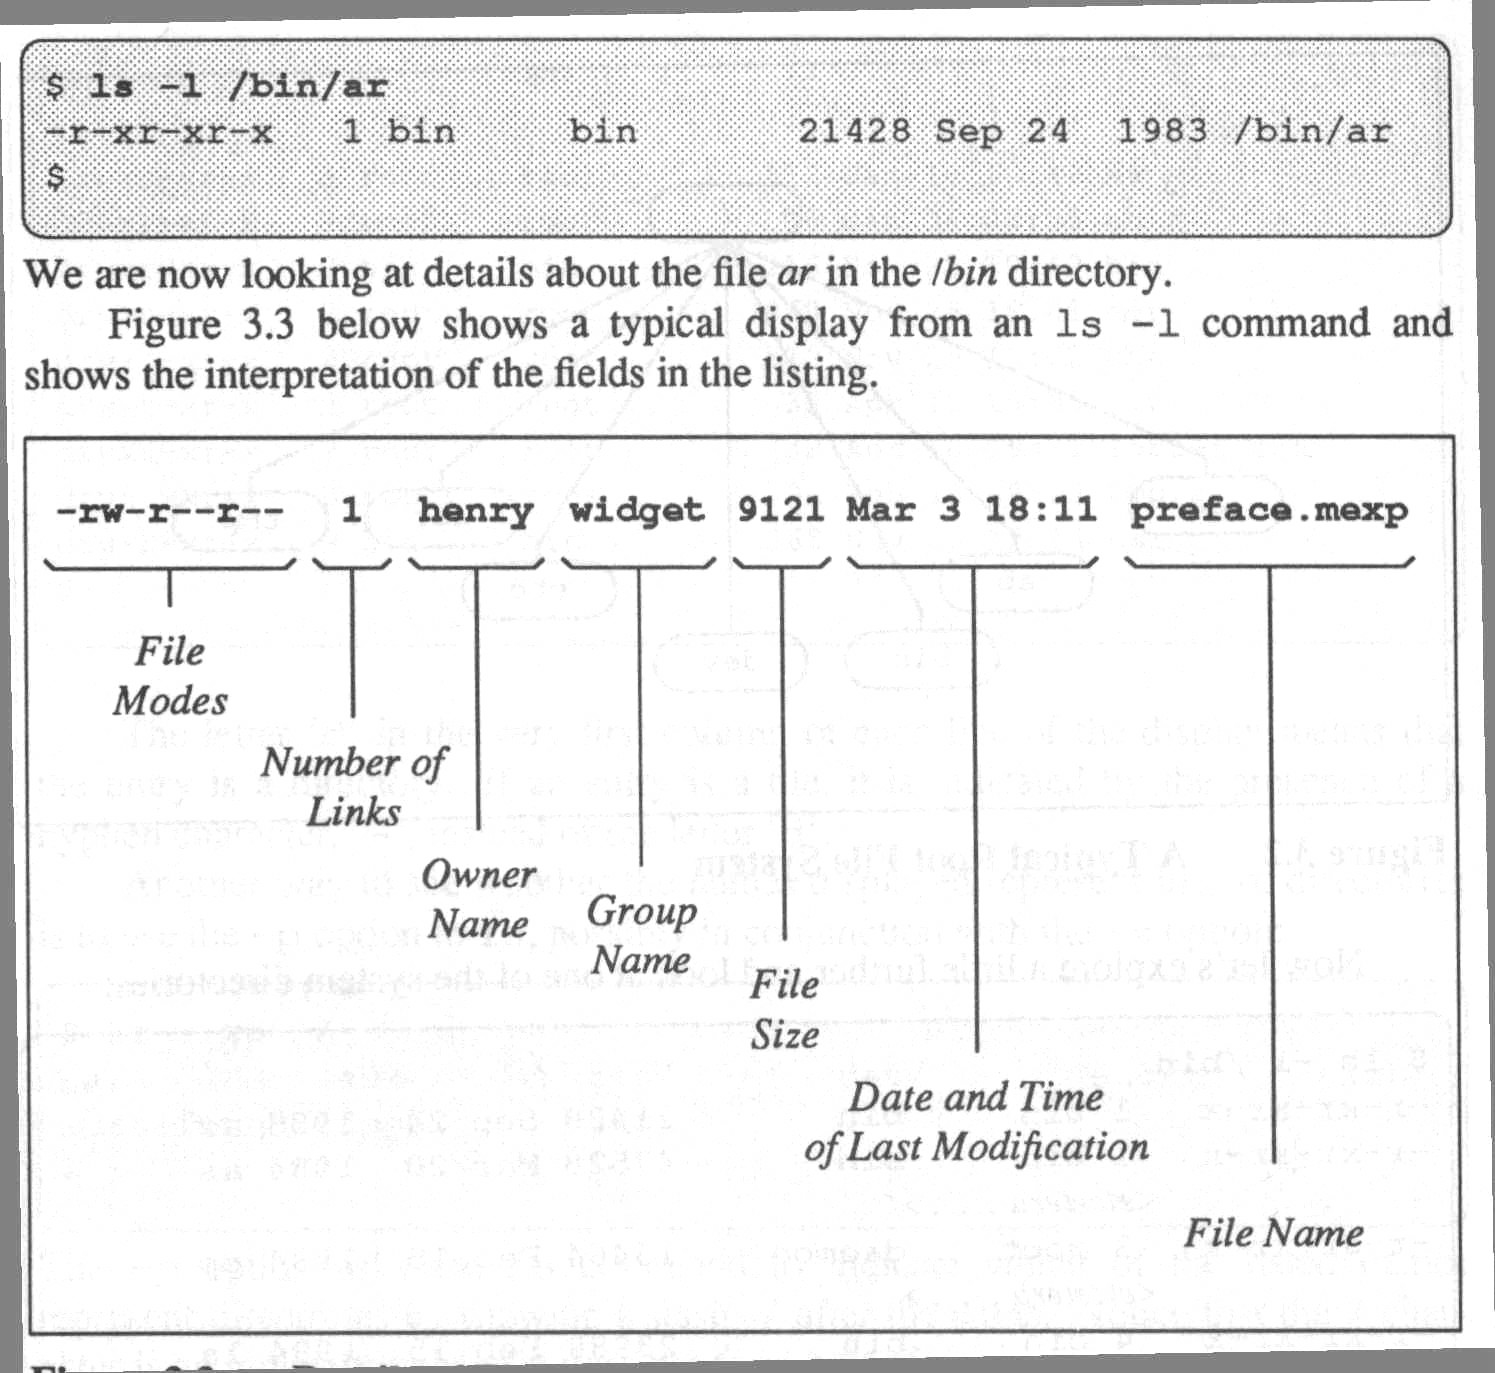
\includegraphics[scale=0.3]{ls}
	\subparagraph{Overlapping} If all/other have rwx, but everyone else has nothing, owner and group cannot rwx, unless the Unix system interprets other as all.
	\paragraph{Archives} TAR, GZIP \& GUNZIP. Archive is a collection of files combined into one file, often compressed. tar combines, gzip compresses. 
	\subsection{Redirection}
	\paragraph{Output} $>$ redirects STDOUT to a text file
	\\ $>>$ appends STDOUT to a text file.
	\paragraph{Input} $<$ takes all input from a file
	\\ To redirect something specific, can prefix by file descriptor, i.e. prog 2$>$errors, redirects errors from prog to errors file.
	\paragraph{Piping/Chaining}
	\begin{enumerate}[.]
		\item Piping commands: redirects STDOUT to another program. i.e. (ls $|$ more) paginates ls output
		\item Doing multiple commands in SUCCESSION: (ls ; echo hi) does ls then echoes hi
		\item Doing multiple commands at ONCE: (ls \& echo hi) does ls and echo at the same time
	\end{enumerate}
	\subsection{Quotes}
	\begin{itemize}
		\item \` \ nested execute symbol \`  \ , executes what's in between first $\to$ string
		\item \textquotesingle as is \textquotesingle 
		\item \textquotedbl pre-process \textquotedbl
		\end{itemize}
	\paragraph{Escape Characters}
	\begin{itemize}
		\item $\backslash$ $\gets$ escape character
		\item $\backslash$n new line
		\item $\backslash$t tab
		\item $\backslash$a bell (noise)
		\end{itemize}
	\subsection{Editors} Command line text editors allow for creation/editing of files at CLI. 
	\begin{itemize}
		\item vi, one of the original ones on Unix, hard to learn. Available on every Unix machine.
		\item pico, simple, based on pine mail client, available on most
		\item emacs, popular, powerful, heavyweight
	\end{itemize}
	There are also graphical text editors.
	\paragraph{Vi}
	Different modes: 
	\begin{itemize}
		\item Edit (i, a, o, O, etc.)
		\begin{itemize}
			\item Edit text
			\item Can press any char
			\item Some vis let you use arrows
		\end{itemize}
		\item Escape Mode (ESC)
		\begin{itemize}
			\item Stops edit
			\item Can use arrow keys
			\item Can use special one letter commands (i,a,h,j,k,l,etc.)
		\end{itemize}
		\item Command Mode (:)
		\begin{itemize}
			\item Can save, load, quit, etc
		\end{itemize}
	\end{itemize}
	ESC: \begin{itemize}
		\item dd deletes a whole line
		\item x deletes current char
		\item r replaces current char by next char types
		\item / to search
	\end{itemize}
	Command: \begin{itemize}
		\item w writes
		\item q quites
		\item wq both
		\item q! quit without saving
		\item e filename to edit file
	\end{itemize}
	\subsection{Regular Expressions} Some commands/editors allow you to search text patters, known as regex. See grep, sed and awk in 3.1 for info about those commands. 
	\paragraph{Examples}
	\begin{itemize}
		\item grep -i \textquotesingle \textasciicircum [aeiouy]\textquotesingle text , want first letter to be a vowel
		\item \textquotesingle [aeiouy]\$ \textquotesingle , want last letter to be vowel
		\item \textquotesingle [aeiouy]\{2,\} \textquotesingle \{min,max\}, want it at least 2 times, 2 vowels next to each other
		\item \textquotesingle \textasciicircum.e \textquotesingle, Start with anything then an e
		\item \textquotesingle \textasciicircum e|a \textquotesingle, start with e or a
		\item \textquotesingle \textasciicircum [a-e] \textquotesingle, start with anything from a to e on unicode table
	\end{itemize}
	\section{Bash Scripts} Scripts are collections of commands grouped in a file to execute in a sequence. Not compiled, interpreted. Run from top to bottom, can alter flow with if statements and loops. Can also create functions (before called). \# indicates a comment. Scripts sensitive to spaces. Good uses for scripts: 
	\begin{itemize}
		\item Backups
		\item Startups
		\item Scheduled
		\item Maintenance
		\item Programmer
	\end{itemize}
	\paragraph{Boot \& Login Scripts} Modify OS environment. Boot made by root for all users, login scripts created by users for themselves. At login, shell looks for default login script.
	\subparagraph{Login Scripts} Used for:
	\begin{itemize}
		\item Configure UI (prompt, color)
		\item TERM communication method, how server speaks to computer
		\item Routines
		\end{itemize}
		In Bash, to change your prompt:
		\\ PS1=``Something here"
		\\ Aliasing commands
		\\ alias lsa=\textquotesingle ls -a\textquotesingle
		\subparagraph{PATH}
		Set of directories a shell searches for executables, separated by (:)
	\paragraph{Command-line Scripts} Created by users to automate command-line things. Everything is a text file, text files can be executed, just add x permission using chmod. Launch a script in current directory using ./myScript
	\subsection{Shell Scripting}
	Start off your script with the sha-bang \#!, to show that script is directly executable and specify shell language/path. \#!/bin/bash
	\paragraph{Variables} 3 kinds in a shell script
	\begin{itemize}
		\item Environment Variable, used to customize OS, used by shell
		\item User-created, created by script itself
		\item Positional Parameters, store what was used to start script
		\end{itemize}
		\subparagraph{Positional Variables}
		\begin{itemize}
			\item \$\# number of args on command line
			\item \$- options supplied to shell
			\item \$? exit val of last command executed
			\item \$\$ process number of current process
			\item \$! process number of last command done in background
			\item \$n argument on command line, n=1-9
			\item shift shifts all arguments by 1, lose \$0, but get \$10 
			\begin{itemize}
				\item \$0 name of shell/program
				\item \$* all args on command line as 1 string
				\item \$@ all args, separately quoted with spaces
			\end{itemize}
			\end{itemize}
			Declaring variables: Just write x=10
			\subparagraph{Some Default Variables}
			\begin{itemize}
				\item \$HOME
				\item \$SHELL
				\item \$TERM
				\item \$USER
				\item \$PWD
				\end{itemize} 
		\paragraph{Reading} Use the \textit{read} command to read a string from STDIN. i.e. read name $\implies$ \$name now stores whatever string the user typed.
		\subparagraph{Capturing Complex Output} If you want to parse multiple args from a command: 
		\\ set \` \ date \` \ will store output in \$n (\$1,\$2, $\ldots$). Will erase data already there.
		\paragraph{Arithmetic} Use, either expr, bc or tell Bash it's math. To make Bash treat Strings as a number, do: 
		\\ \$((1+1)) or \$[1+1]
		\\ For fractions, use bc. echo \textquotedbl scale=\#ofdecimals;3/4 \textquotedbl | bc
	\paragraph{Conditionals} Use the test command to evaluate an expression or case. Bash does not require the test command though. Can evaluate at file, string or integer level.
	\subparagraph{File Tests}
	\begin{itemize}
		\item -r file : exists + readable
		\item -w file : exists + writable
		\item -x file : exists + executable
		\item -f file : exists + regular
		\item -d name : exists + directory
		\item -h or -L file : exists + link
		\item etc.
		\end{itemize}
	\subparagraph{String Tests}
	\begin{itemize}
		\item -z string : string length zero (Not null, but 0)
		\item -n string : length non-zero
		\item string1 = (or ==) string2 : strings identical
		\item string1 != string2 : not identical
		\item string : not null
		\end{itemize}
	\subparagraph{Integer Tests}
	\begin{itemize}
		\item n1 -eq n2 : integers equal
		\item n1 -ne n2 : not equal
		\item n1 -gt n2 : $n1>n2$
		\item n1 -ge n2 : $n1 \geq n2$
		\item n1 -lt n2 : $n1<n2$
		\item n1 -le n2 : $n1 \leq n2$
		\end{itemize}
	\subparagraph{if Statement} ~
\begin{lstlisting}[language=bash]
if _condition_
then
	stuff
elif _condition_
then
	stuff
else
	stuff
fi
\end{lstlisting}
\subparagraph{case Statement}~
\begin{lstlisting}[language=bash]
case what_to_check in

condition1) action1;;
condition2) action2;;
*) else_action;;
esac
\end{lstlisting}
\paragraph{for Loop} Iterates.
\begin{lstlisting}[language=bash]
for var in list
do
	stuff
done
\end{lstlisting}
\paragraph{while Statement} Continues until statement false.
\begin{lstlisting}[language=bash]
while condition
do
	stuff
	continue (back to beginning)
	break (end loop)
done
\end{lstlisting}
\paragraph{Functions}
\begin{lstlisting}[language=bash]
function() {
stuff
}
\end{lstlisting}
Functions must be declared before called.  

\paragraph{Etc.}
Good practice to exit scripts with exit codes, 0 for no errors, 1-255 for errors.
\section{C}
\subsection{About C}
\paragraph{History}
Successor for B and BCPL. Creation parallel to development of early Unix OSes (1969-1973). Good because it's portable and can access hardware, lower level language. C++, successor to C. Java, C\# and JavaScript based on C. 
\paragraph{Comparison to Java}
Same as Java for: 
\begin{itemize}
	\item If
	\item For loop
	\item While/do-while loop
	\item Methods (called functions)
	\item Types : int, float, double, char
	\item Variable creation
	\item Mathematical and logical expressions
	\end{itemize}
	Mathematical operators (+,*, etc.) exact same as Java. Type casting sometimes implicit, like int $\to$ float, but can cast specifically like in Java.
\\Similar to Java for:
\begin{itemize}
	\item Arrays
	\item References (pointers)
	\item Main method (main function)
	\item Scope
\end{itemize}
\textbf{Different} from Java for:
\begin{itemize}
	\item Strings
	\item No objects (but there are modules)
	\item Libraries
	\item Pre-processor, compiling in different languages, Eng/Fr, etc.
\end{itemize}
\subsection{C Program Structure}
\begin{lstlisting}[language=c]
#include <stdio.h> // C library, always need stdio.h
int main (int argc, char *argv[]){ 
//main function, *argv[] are command-line parameters
	printf("Hello World \n"); //prints
	return 0; //return if there's an error or not to calling program
}
\end{lstlisting}
int argc consists of number of arguments at command-line (including argv[0], prog name)
\\ char *argv[], each cell has one command-line parameter.
\subsection{Format of Types for Strings/printf,etc.}
To input a char or String or int or something else indirectly into printf, have to declare the spacing of it with \%. 
\begin{align*}
	\% \overbrace{\#}^{\text{int, optional. How much space?}}\underbrace{c}_{\text{type, c=char, s=string, d=int, f=float}}
\end{align*}
More control codes: 
\begin{itemize}
	\item \%d or \%i : signed integer
	\item \%x : unsigned hexadecimal
	\item \%u : unsigned decimal
	\item \%E : double of form m.ddExx
\end{itemize}
Ex. 
\begin{lstlisting}[language=c]
printf("user %s hello \n", name);
\end{lstlisting}
Prints user bob hello, if bob stored in name. \%10s represents 10 white spaces, first x amount with variable. If you write less numbers than the length of the String, it won't truncate, will just use length, like \%s.
\\ For floats, \%5.2f, 5 is total amount of numbers, .2 is number after decimal.
\\ x++ increments after operation (x++-3=x-3+1), ++x increments before (++x-3=x+1-3)
\subsection{Libraries \& Functions}
\paragraph{Functions} If you want to write the code for a function after calling it, have to use a function prototype, that is, declare the function at the beginning, but write the code later (telling compiler to look for the function). Names of variables in prototype don't have to match, but return type has to match.
\begin{lstlisting}[language=c]
void add (int,int);
.
.
.
void main(void){
int z = sum (5,10);
}
.
.
.
void add (int a, int b){
int x=a+b
}
\end{lstlisting}
You \textbf{CANNOT} overload functions in C, counts as conflicting signatures (function name, return type and parameters).
\paragraph{What are libraries?} Toolbox for common routines that are often optimized and speed up development time. They allow you to create reusable code to share with others, but can make code size large. Include at beginning of code. Can also include things like headers or c code.
\\ Made up of .h, the header file with function prototypes \& typedefs and .o, compiled from .c without a main
\paragraph{stdio.h}~
\begin{tabularx}{\textwidth}{|X|X|X|}
	\hline \textbf{function} & \textbf{example(s)} & \textbf{use}
	\\\hline printf(\textquotedbl stuff\textquotedbl) & printf(\textquotedbl Hello World\textquotedbl); printf(\textquotedbl \%d \textquotedbl, 25); & Prints to screen
	\\\hline scanf(a) & scanf(\textquotedbl \%d \%d \textquotedbl, \&age1, \&age2); & scans variables from user
	\\\hline int getchar(void) & & gets one char from STDIN
	\\\hline int putchar(int) && displays one char to STDOUT
	\\\hline gets(array) && reads string into array
	\\\hline fgets(char array, int size, *stream) && reads string of certain size from file into array
	\\\hline int getc(any stream)/getchar(STDIN only); && read one char
	\\\hline int puts(*string) && place char
	\\\hline remove (*file) &&
	\\\hline rename(*file1, *file2) & rename(``text1'',``text2'')& Files are Strings
	\\\hline fopen (filename, mode [rt,wt,at]) & fopen (text.txt, \textquotedbl wt \textquotedbl); & opens file ptr
	\\\hline fprintf(ptr, description, vars) &&
	\\\hline fscanf(ptr, description, \&vars) &&
	\\\hline feof(ptr) && 0, 1 if end of file
	\\\hline fclose(ptr) && closes file read/write, adds EOF char(write)
	\\\hline fflush(ptr) && empties buffer without writing
	\\\hline
\end{tabularx}
scanf anomaly: Does not process carriage returns properly, viewed as string or char. When you read numbers, carriage return is left in input buffer! You should scan numbers after all strings, unless you have intermediate garbage (char) scans to scan leftover carriage returns.
\\scanf limiting vs gets, need specific amount of args/words, get gives you the whole line.
\\sprintf \& sscanf do same thing as printf \& scanf, except they return how many they were able to read/print
\paragraph{stdlib.h}~
\begin{itemize}
	\item NULL 0
	\item EXIT\_FAILURE 1
	\item EXIT\_SUCCESS 0
	\item rand(void), 0 to RAND\_MAX
	\item system(string), sends command to system, command-line (launches a new shell), returns int, exit code (can check if BASH had an error)
	\item atof(string), ascii to float
	\item atoi(string), ascii to integer
	\item abs(int), abs val
	\item exit(int), 1 or 0
\end{itemize}
\paragraph{math.h}
\begin{itemize}
	\item sqrt(double);
	\item power(base,exponent);
	\item abs(int);
	\item fabs(double);
	\item floor(double);
	\item ceil(double);
	\item sin, cos, tan, asin, etc.
\end{itemize}
\paragraph{ctype.h}
\begin{itemize}
	\item toupper(int);
	\item tolower(int);
	\item isalpha(int);
	\item isalphanum(int);
	\item isdigit(int);
\end{itemize}
\paragraph{string.h}
\begin{itemize}
	\item strlen(string)
	\item char *strcpy(char *dest, char *src), copies string
	\item char *strcat(char *dest, char *src), concatenates string
	\item strcmp(char *s1, char *s2), compares contents of 2 strings (instead of addresses), 0 if same
	\end{itemize}
\subsection{Compiling} Use gcc to compile. Default executable name is a.out.
\\ 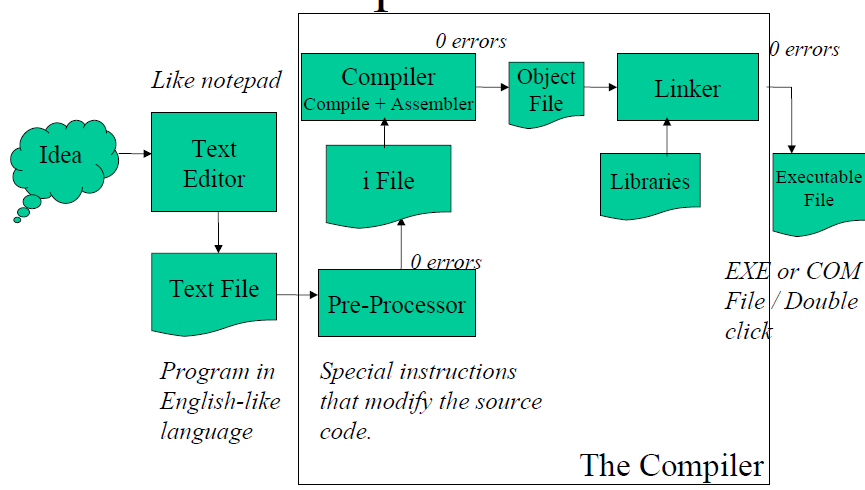
\includegraphics[scale=0.5]{cco}
\paragraph{C Files}
\begin{itemize}
	\item Source files: file.c (program). file.h (header, shared)
	\item Pre-processed: file.i
	\item Object \& assembler: file.o, file.s
	\item Executables: file, a.out
	\end{itemize}
\paragraph{GCC Syntax}
GCC is the GNU C Compiler.
\\ gcc -o executablename sourcefilenames
\\ Variations include:
\begin{itemize}
	\item gcc -E main.c, makes .i file
	\item gcc -S main.c, makes assembler(.s) code
	\item gcc -c main.c, makes object(.o) code
	\item gcc main.c, makes a.out
	\item Extra switches:
	\begin{itemize}
		\item -o filename, specify name of output
		\item -v verbose
		\item -w suppress warnings
		\item -W extra warnings
		\item -Wall all warning messages
		\item -O1 optimize for size and speed
		\item -O2 optimize even more
	\end{itemize}
\end{itemize}
\paragraph{C Types} ~\\
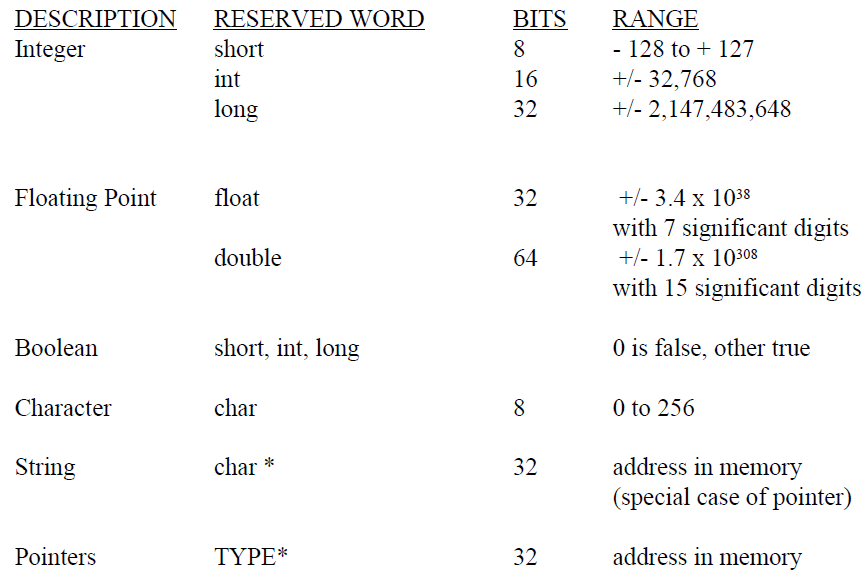
\includegraphics[scale=0.5]{ctyp} Notice that booleans don't really exist (they're just ints) and Strings are char pointers. Strings end with a null.
\paragraph{Booleans}
$0=$ false, anything else is true. Greatly affects if statements, as your condition can solely be math and it'll check if it's 0 or not. So you won't have a compilation error for something like x=5, but very different from x==5.
\paragraph{Strings} Strings are just character arrays terminated by a null. Can declare some like: char *x = \textquotedbl Bob \textquotedbl;
\\ Cannot scanf into a *, as * constant/fixed to what they were when declared. When scanning into a char array, don't use \&.
\subparagraph{Arrays} int x[10];
\\ Can also declare literally and also leave extra commas to denote extra spaces.
\\ int x[]=\{1,2,3,4,,,,,,\}
\\ In C, you can go past the indexes of an array. 
\\ char x[10]; $\to$ [char][char]$\ldots$[char]
\\ char *y[10]; $\to$ [ptr][ptr]$\ldots$[ptr]
\paragraph{Declaring a Variable}
~\\ SCOPE MODIFIER TYPE VAR\_NAME;
\\ SCOPE is static, extern or not used. MODIFIED is unsigned(no signed bit), short($\frac{1}{2}$ bits), long($2\times $ bits) or not used. TYPE, a built in type.
\\ Variables are \textbf{NOT} defaulted to 0.
\\ Can also chain assignments, int a,b,c,d=4;
\\ Can also declare constants
\\ int const a = 1; or const int a = 2;
\\ Variables declared at either top of file (global variable) or in a function (local variable). Global variables are positionally global, accessible to everything below it. Only one copy of a global variable exists. Global variables should be avoided if not needed, hard to debug and not considered clean.
\\ Variable preference: block vars $\to$ local vars $\to$ global $\to$ extern $\to$ error/compiler error
\subsection{Pointers} Special unsigned integer storing an address. Can reference anything really. Mainly used to point to a variable or location in RAM. Note that a pointer is not the same thing as a reference, a reference is a Java concept.
\paragraph{Pointer Operations}
\begin{itemize}
	\item \& unary/monadic operator, gives address of variable
	\item * indirection/dereference, gives contents of object pointed to, declare pointers using *
	\end{itemize}
	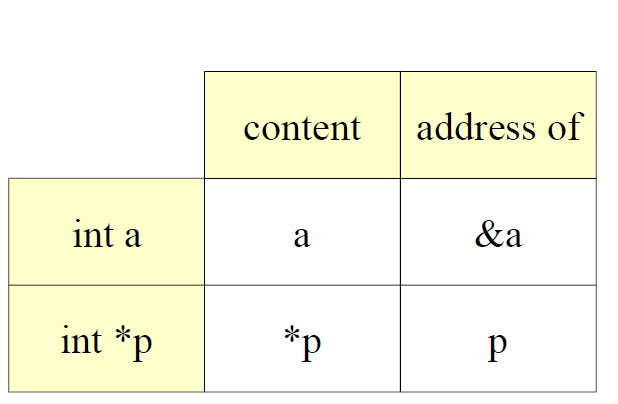
\includegraphics[scale=0.5]{pont}
\begin{lstlisting}[language=c]
int a,b,*p;
p=&a
\end{lstlisting}
p will now point at a's address.
\begin{lstlisting}[language=c]
int a, b;
int *p;

a = 5;
b = 10;
p = &a; // p is pointing to a
*p = 6; // Value of a is now 6
p = &b; // p is pointing to b
*p = 11 // Value of b is now 11;
\end{lstlisting}
Giving type to your pointer means it can only point to that type. void * can point to anything.
\begin{lstlisting}[language=c]
char* x,y,z; // all vars are char*
char x, *y, z; // only y is char*
\end{lstlisting}
Pointers are not constant, can change (since they're variables), unless you declare explicitly, like a String (then it's static/literals).
\begin{lstlisting}[language=c]
char *string = "bob"; // Literal / static
char array[10]; // Variables / dynamic
\end{lstlisting}
\paragraph{void* Pointers} void pointers can point to anything, anywhere. They are the bit-size of addresses.
\begin{lstlisting}[language=c]
int x=5,y;
void *p;

p=&x;
y=*p; // Warning
y=*(int *)p; // Cast
\end{lstlisting}
\paragraph{Arrays} When you create an array in C, you're allocating a block of memory and creating a pointer to the first element of the block (like using malloc).
\paragraph{Strings}
\begin{lstlisting}[language=c]
SCOPE MODIFIER char* VARNAME = "characters"
\end{lstlisting}
Going to different indices in a String/pointer, add the offset.
\begin{lstlisting}[language=c]
*(str+2); // 3rd char of the String
\end{lstlisting}
If we don't terminate a String by a null, it will keep going until it hits a null
(when trying to read it).
\subsection{Parameter Passing}
\begin{itemize}
\item Primitive types are passed by value. You get a local copy of the variable for the function.
\item Arrays are passed by reference, affects the whole program if you change them in a function (same for pointers).
\item Passing a parameter with the unary (\&) operator makes it pass as a pointer, which is how scanf works.
\item You cannot make a function that swaps primitives \textbf{unless} you use pointers to the primitives.
\end{itemize}
\subsection{Switch Statement}
Check variable for equality against a list, check for each switch case.
\begin{lstlisting}[language=c]
switch(expr){
    case const-expr:
        printf("hi");
        break; // optional

    case 2:
        printf("It's a 2!");
        break;

    default: //optional
        printf("None");
}
\end{lstlisting}
\subsection{Reading/Writing to a File}
Files/text, displayed in 2D but actually 1D structure, like an array. The Disk actually consists of the FAT (File Allocation Table), a bunch of name of files and pointers. To read/write to a file, need to get a pointer to disk.
\\ Modes for opening files (fopen):
\begin{itemize}
\item r: opens file in read mode
\item w: write mode (if none, creates. If existing, deletes)
\item a: append mode (if none, creates)
\item r+w: read and write (not destructive)
\end{itemize}
\lstinputlisting{C/fileio.c}
\paragraph{Named Space}
Location where data is stored, these locations have names.
\subsection{Pre-processor}
The pre-processor takes care of things like directives. Takes the source.c file and makes it into a source.i file, which is then fed into the compiler.
\paragraph{2 types of include}
\begin{lstlisting}[language=c]
#include<stdio.h> // <> -> in library folder
#include "path/textfile" // ""->path
\end{lstlisting}
What include does is basically insert source file at that location.
\paragraph{Define}
\begin{lstlisting}[language=c]
#define NAME EXPRESSION //format
#define MACRO EXPRESSION //format
\end{lstlisting}
EXPRESSION consists of any legal C expression. MACRO follows: NAME(PARAMETERS), with params being a comma separated list. Convention is to name something defined in all caps so we know it was defined using \#define. Notice that FILE is written all in caps, was defined in stdio.h. 
\begin{lstlisting}[language=c]
#define LIMIT 10
int array[LIMIT]; // Allows something like this -> array[10]
#define BOOLEAN int
#define TRUE 1
#define FALSE 0
// Macros
#define INC(x) x++
#define MAX(A,B) (A<B)?B:A
// becomes B if true: A if false
\end{lstlisting}
\paragraph{Define vs const} const int a = 5; can be typechecked(safer) by compiler, but uses extra memory.
\paragraph{Ifdef} Check if something is/isn't defined. Must end by \#endif. Good to protect against defining same thing twice. Can also include stuff like function prototypes/code. Can put these in the middle of your code. Useful for writing a multilingual program. ifdef the language everywhere and print corresponding language's output. If the program defines that language in the beginning, you'll get the program in the language.
\begin{lstlisting}[language=c]
#ifndef AGE // If age isn't already defined (possibly from include)
#define AGE 20
#else // optional
#endif
\end{lstlisting}
\paragraph{Using the Pre-processor for Collaboration} Multiple programmers on one team, all working on the same project.
\paragraph{Single Source File Programming} Have all the .c files in the same directory, include them all in main.c, single source because only one .i file results from this. Everything except local variables are global (no named spaces), all compiled in same place.
\paragraph{Header Files}C code is separated into source (.c) files and header (.h) files. They contain:
\begin{itemize}
\item Pre-processor commands
\item Global variable declarations (extern)
\item Function prototypes
\end{itemize}
\paragraph{Extern Modifier} To use a variable from another file/source, write extern type varname; at the top of source code (can put in header file to know which vars are supposed to be global). The extern modifier lets a named-space access data in another named-space (compiler will look in other source files, can only have one other declaration of this variable in all yoru source files). Assumed on functions.
\begin{lstlisting}[language=c]
// Math.h would look something like:
extern double PI;
int factorial(int n);
\end{lstlisting}
\paragraph{Modular Programming} Everyone has their own (hidden) named space. Make a .c source file, a .h header file, which includes function prototypes for functions that you allow others to use in their source. .h files included in sources that need functions from those parts (main should have .h for each file).
\begin{lstlisting}[language=bash]
gcc -c f1.c # Gives resultant f1.o from preproc
\end{lstlisting}
.o files are semi private, have to reverse binary/assembler to see. To compile the final project:
\begin{lstlisting}[language=bash]
gcc main.c f1.o f2.o
\end{lstlisting}
Lots of .o files to include. Can make a BASH script to do this. Another way of fixing stuff is using a \textbf{makefile}.

\subsection{GNU Tools}
\paragraph{Make} An automated build utility. Determines which pieces need to be recompiled and issues corresponding commands. Make can be used with any language. Can use variables like in BASH.
\\ Advantages: Allows us to define multiple ways to compile, has scripting ability. Greatly speeds up compile time with selective compilation. 
\begin{lstlisting}[language=bash]
myProg: main.o f1.o f2.0 # If these exist, exec line below
    gcc -o myProg main.o f1.o f2.o
    # Indents mandatory, can put multiple commands
main.o: main.c f1.h f2.h
    gcc -c main.c
misctag: #i.e. make misctag, make clean to remove compiled files
\end{lstlisting}
Makefile reads from bottom to top. Also checks date. If source code is newer than compiled file, will recompile that section, i.e. main.c newer than main.o, recompile main.o. Make has an implicit rule where it will update .o file from corresponding .c file (i.e. you don't need to write the .c file in the conditions if it has the same name), but it's better not to use the implicit rule.
\paragraph{Terminology}
\begin{itemize}
\item 
\textbf{Unit}: collection of files compiled into a single .o file. (.c and .h)
\item 
\textbf{Project}: collection of units linked into a single executable file. (collection of .o files)
\item \textbf{make}: GNU program that compiles projects
\item \textbf{makefile}: text file containing script
\end{itemize}
In order to use make, have makefile in the source directory and run ``make''.
\paragraph{Repository} Database that stores all versions of files you've been working on. Lets you revert to previous versions and branch out and experiment with different ways of developing files. Repositories store any kind of file. Also lets you merge a source file if 2 people edited it at the same time and can password lock source files.
\\ Repository Tools:
\begin{itemize}
\item RCS (root based)
\item CVS (root based)
\item SVN
\item GIT (peer based)
\end{itemize}
\paragraph{Root-Based Code Repositories} Code is shared online, users have access to it.
\paragraph{Peer-Based Code Repositories} Everyone has their personal part, which is staged (git add <files>) which gets committed to the local repository (git commit) and pushed to the remote repository (git push)
\paragraph{Using Git}
root(1.1)$\to$trunk(1.2)$\to$branch(1.2.1)$\to$tip(1.2.2) or trunk(1.2)$\to$tip(1.3), tip is the most recent version, trunk is intermediate, root is original and branch is a separate version/direction.
\begin{lstlisting}[language=bash]
# Move to directory with code to manage with git
cd /project/ass1/source
git init #Initializes repository
# For remote repo download:
git clone git@github.com:repo.git
# Pick files (Stage)
git add f1.c f2.c
git commit # Checks in
\end{lstlisting}
Basic Git Commands:
\begin{tabularx}{1.0\linewidth}{|X|X|}
  \hline
  \textbf{Command} & \textbf{Info}
  \\\hline git init  & setup repo
  \\ \hline git add & add files for next commit
  \\ \hline git commit & commit queued files
  \\ \hline git commit -m ``Message'' & Add message to commit
  \\ \hline git push & push commit(s) to remote repo
  \\ \hline git pull & fetch changes from remote
  \\ \hline git clone & clone repo into local dir
  \\ \hline git status & show uncommited changes
  \\ \hline git rm & remove file from repo
  \\ \hline git mv & move file within repo
  \\ \hline git diff & differences between multiple commits
  \\ \hline git log & log of commits
  \\ \hline
\end{tabularx}
Add files to .gitignore to ignore specific files.
\\ Branching
\begin{tabularx}{1.0\linewidth}{|X|X|}
  \hline \textbf{Command} & \textbf{Info}
  \\ \hline git branch new\_branch & create new branch
  \\ \hline git branch -b new\_branch & create and switch to new branch
  \\ \hline checkout master & switch back to master
  \\ \hline git merge branch2 & merge work, all commits from branch2 to one commit in current
  \\ \hline git rebase branch2 & rebase your current branch off updated branch2, incase unrelated things updated in branch2. Good to rebase before merging, to see if anything breaks before merging.
  \\ \hline git branch -d branch2 & delete branch
  \\ \hline
\end{tabularx}
Tagging (adding releases)
\begin{tabularx}{1.0\linewidth}{|X|X|}
\hline \textbf{Command} & \textbf{Info}
  \\ \hline git tag -a name& Add tag with this name
  \\ \hline git tag -l & Lists tags
  \\ \hline git push --tags & Push tags to remote
  \\ \hline
\end{tabularx}
Modifications:
\begin{tabularx}{1.0\linewidth}{|X|X|}
  \hline \textbf{Command}& \textbf{Info}
  \\ \hline git commit --amend & Change last commit
  \\ \hline git reset HEAD file\_name & Unstage staged file
  \\ \hline git checkout --file\_name & Unmodify modified file
  \\ \hline
\end{tabularx}
\paragraph{GNU Debug (GDB)}
A software bug is an error/flaw/mistake/failure/fault in program preventing it from working as intended. Bugs can exist at design level or source code level. Side-effects: incorrect answer, crash application, loss of data, loss of money, loss of life.
\\ \textbf{Debugging} = finding the source of a bug \& fixing it. Hardest part is finding the problem (becomes increasingly difficult when source is large). Analyzing code sometimes won't cut it. You might need to run the program. Debuggers help the debugging process. Allows programmer to run program in different mode. Many new features available to programmer. Can see what line causes a program crash, analyze application line by line, consult content of memory. Most languages have a debugger. printf is useful, but can't do everything that a debugger can (pause program, list source code, print data, jump to a line of code).
\\ GDB is part of the GNU OS, can be used for C, C++, Objective-C, Fortran, Java and Assembly programs.
\\ To use GDB, compile executable with the -g flag. Compiles the program with extra info, like source code and symbol table. 
\begin{lstlisting}[language=bash]
gcc -g -o HelloWorld HelloWorld.c
# Then call gdb on the executable
gdb HelloWorld
# You will now be in "gdb" mode
(gdb) help # Gets list of available commands
# Can also get help on specific command
(gdb) help breakpoints
\end{lstlisting}
To look at Source code, use the list command. Takes either a filename and line bumer or function name or just line number.
\begin{lstlisting}[language=c]
(gdb) list main.c:10
set listsize # Changes size of a list
(gdb) run # Runs code until crash
# Can also run line by line
(gdb) step
(gdb) next 
\end{lstlisting}
Step \& next both do the same thing, but step will step into a function call, next will execute the function call, but not step through.
\\ More GDB commands
\begin{tabularx}{1.0\linewidth}{|X|X|}
  \hline \textbf{Command}&\textbf{Info}
  \\ \hline quit & end gdb
  \\ \hline list & shows 10 lines (default)
  \\ \hline list n,m & show lines n to m
  \\ \hline list function & show function
  \\ \hline run & runs program
  \\ \hline ctrl-c (during run) & interrupt program
  \\ \hline run -b <in> out & redir in \& out to prog
  \\ \hline backtrace & see run-time stack
  \\ \hline whatis x & show x's declaration
  \\ \hline print x & show value of x
  \\ \hline print fn(y) & execute fn with y
  \\ \hline print a @ n & print n elements of array a
  \\ \hline break n & puts a breakpoint at line n, stops there during run
  \\ \hline break n if EXPR & break at line n if true (i.e $i=99$ for loop), can do same for fn
  \\ \hline break fn & interrupt program at function call
  \\ \hline break filename:lineno & break at line number of source file
  \\ \hline continue & continue after break
  \\ \hline watch EXPR & stop program when expr is true
  \\ \hline set variable NAME = VALUE & change contents of variable
  \\ \hline ptype NAME & pretty print of NAME (as struct)
  \\ \hline call fn(y) & execute fn with y
  \\ \hline info breakpoints & gives info about breakpoints
  \\ \hline delete n & deletes breakpoint n
  \\ \hline delete & deletes all break points
  \\ \hline clear n & clear break or watch on line n
  \\ \hline disable n & disables break on line n
  \\ \hline enable n & enables break on line n
  \\ \hline enable once n & turn on once
  \\ \hline where & produce backtrace
  \\ \hline
\end{tabularx}
\paragraph{DDD}A graphical front-end for command-line debuggers like GDB, DBX, JDB, Python debugger, etc. Can do four things:
\begin{itemize}
\item Start program
\item Make program stop on conditions
\item Examine what happened
\item Change things in program
\end{itemize}
\paragraph{Lint} Lint originally flagged suspicious/non-portable constructs/bugs in C. Now the name signifies any tool reporting suspicious behavior like:
\begin{itemize}
\item Variables being used before set
\item Conditions that are always true/false
\item Calculations whose result is likely to be out of range of values representable by type used
\end{itemize}
\paragraph{GProf} Program can be unacceptably slow, takes longer to complete operation than desired. Program needs to be optimized, so it can accomplish same tasks with less resources. Behavior of program should be unchanged. We need to be able to identify portion that is slow.
\paragraph{Definitions of Slow}
\begin{itemize}
\item \textbf{Big-Oh} Logical speed of algorithm. Pro: Independent of hardware. Con: Long to do on large pieces of code.
\item \textbf{Clock Time} Actual speed corresponding to hardware (MHz, RAM, devices). Pro: Can be automated. Con: Hardware dependent.
\end{itemize}
\paragraph{Profilers}Dynamic performance analysis tools. Lint are static analysis tools. Profilers record data as application executes. Usually tells you what part is slow/uses a lot of memory.
\paragraph{Using GProf}
\begin{lstlisting}[language=bash]
gcc -pg file.c #Compile file with timechecks
\end{lstlisting}
After running the program, a gmon.out binary file will be created.
\begin{lstlisting}[language=bash]
gprof -b a.out gmon.out > statsfile # Read results
\end{lstlisting}
The output will be messy/long, so better to redirect to a text file.
\\ Options:
\begin{itemize}
\item -b not verbose
\item -s merge all gmon files
\item -z table of functions never called
\item -a don't print statically declared (private) functions
\item -e funcname, don't print info about this function
\item -E funcname, like -e, but time spent in function won't be printed
\item -f funcname, only print specified function and children
\item -F funcname, only time spent
\end{itemize}
\paragraph{Flat Files} Here's a GProf flat file sample, running bubble sort on 100,000 numbers on a relatively slow computer.
\lstinputlisting{C/gprofsample1.txt}
\begin{tabularx}{1.0\linewidth}{|X|X|}
 \hline \textbf{Column}&\textbf{Info}
  \\ \hline \% time & Percentage of time program spent in this function, should add to 100.
  \\ \hline cumulative seconds & Total number of seconds spent executing this function plus time spent in functions above this one.
  \\ \hline self seconds & Number of seconds(or milliseconds) form this function itself. Flat profile sorted by this number.
  \\ \hline calls & Number of times the function was called, blank means none.
  \\ \hline self s/call & Average number of seconds (or ms) spent in the function per call
  \\ \hline total s/call & Average number of seconds spent in this function and its descendants per call.
  \\ \hline name & Name of function. Sorts this alphabetically after self seconds is sorted.
  \\ \hline
\end{tabularx}
\paragraph{Call Graphs}
\lstinputlisting{C/gprofsample.txt}
Primary Line: Describes function
\begin{tabularx}{1.0\linewidth}{|X|X|}
  \hline \textbf{Column}&\textbf{Info}
  \\ \hline index & Entries numbered with integers.
  \\ \hline \% time & Percentage of total time spent in function (includes time spent in subroutines called by function, main should be 100).
  \\ \hline self & Total amount of time spent in function, sohuld be indetical to number in seconds field of flat profile.
  \\ \hline children & Total amount of time spent in calls made by function.
  \\ \hline called & \# times function was called/\# of non-recursive calls form all callers
  \\ \hline
\end{tabularx}
Function's Callers: Function has a line for each function it was called by.
\subsection{Invoking Programs}Already saw that we can call a new shell with the system command. But we can also use int fork();, need \#include<unistd.h>. Fork will make child process, duplicates current program and runs from after the line that forks, with concurrent execution of parent and child processes. Returns PID of child for parent, 0 for child. If parent dies before child, child may terminate prematurely. Need to use wait function with \#include<sys/wait.h>.
\paragraph{Main Program (Driver)} Creates \& manages children, but they do all the work. Fork copies all variables except return val of fork, so you can use if statements to check if child or parent. Since previous variables are maintained, parents can speak to children, but not the other way around (unless you use something like a textfile to communicate).
\paragraph{Waiting for Children}
\begin{lstlisting}[language=c]
int status=0;
int pid = fork();
if(pid == 0){ // Child
    //Do stuff
}
else if(pid<0){ //For failed
    status =-1;
}
else{//Parent
    while(waitpid(pid,&status,0)==0); // Loop until done
}
\end{lstlisting}
\subsection{C Data Structures}
struct, creates a type. Kind of like a class without functions (unless you implement pointers to functions).
\begin{lstlisting}[language=c]
struct STUDENT{
    // Fields
    char name[30];
    int age;
    double gpa;
}x; // Variable name is optional, will create one if specified
// Semi-colon is mandatory though
\end{lstlisting}
We can then use the dot operator.
\begin{lstlisting}[language=c]
x.age=19;
\end{lstlisting}
To declare a struct, we can use a pointer or a literal.
\begin{lstlisting}[language=c]
struct STUDENT z; 
struct STUDENT x[30]; //For 30 students
z.age=20;
// or, using pointers:
struct STUDENT *p;
// Allocates memory the size of STUDENT structure
p = (struct STUDENT*)malloc(sizeof(struct STUDENT));
// Cannot use dot operator here
p->age=20; // Assign age of struct to 20
printf("%d",p->age); // Print age of struct
\end{lstlisting}
We can also nest structures, defining another struct inside the definition of a struct.
\paragraph{Unions}
For polymorphic things, where we represent the same data as multiple types. All data is stored in the same spot (whereas for structs, everything has its own memory). Useful when you want to store something that can be multiple types. Merges variables into a single variable. Can declare unions and structs inside of a function too.
\begin{lstlisting}[language=c]
union NUMBER{
    short int a;
    int b;
    float c;
    double d;
}number;
\end{lstlisting}
In this case,
\begin{lstlisting}[language=c]
number.a=5;
number.b=6;
\end{lstlisting}
will both overwrite the same memory (you should not be modifying multiple parameters of a union, only using the respective one for that case).
\\ We can put unions in structs and structs in unions and whatnot.
\paragraph{typedef Declaration} Can make your own type, i.e.
\\ typedef int boolean;
\\ It can also be used with structs so you don't need to specify structs.
\begin{lstlisting}[language=c]
typedef struct COURSE{
    ...
}nameOfVar;
// Then when creating a COURSE
nameOfVar c206; 
\end{lstlisting}
\paragraph{Enumerated Types}
Contains a list of constants that we can refer to as integers.
\begin{lstlisting}[language=c]
enum days {mon, tue, wed, thu, fri, sat, sun};
\end{lstlisting}
mon has value $0$, tue has value $1$ and so on... Can change to your own values.
\begin{lstlisting}[language=c]
enum days{mon = 1, tue, wed, ...}
// or
enum days{mon = 10, tue = 20, ...}
// then
int x = mon+tue; // x = 30;
\end{lstlisting}
\subsection{Memory}
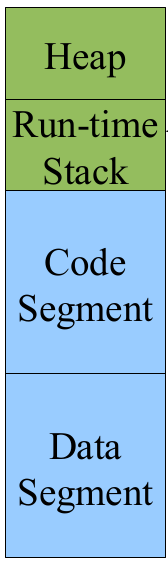
\includegraphics[scale=0.3]{proc} A visual representation of a process. The heap contains dynamic memory, used by malloc and calloc. The run-time stack consists of local variables \& functions.
\paragraph{Dynamic Memory Allocation}
\begin{lstlisting}[language=c]
#include <stdlib.h>
void *malloc(int numberOfBytes);
void *calloc(int repeat, int numberOfBytes);
void *realloc(void *ptr, int numberOfBytes)' 
\end{lstlisting}
calloc initializes all blocks to $0$. Malloc and calloc return a void pointer, so you must cast it before you can use it for a specific type of pointer.
\begin{lstlisting}[language=c]
int *a = (int *)malloc(sizeof(int)*40);
int *a = (int *) calloc(40,sizeof(int));
\end{lstlisting}
sizeof() calculates the size of the data type.
\paragraph{Deallocating}
Use the free() function to release memory.
\begin{lstlisting}[language=c]
void free(void *ptr);
\end{lstlisting}
If you do not release memory after being done with it, you may cause a memory leak (no garbage collector).
\paragraph{Dereference Operator}-> for accessing pointer fields (see structs)
\section{Web}Designed to follow client-server model. The client consists of a device with a browser, loaded with html, CGI and the like. Has input/output. Linked to a web server that accepts packets and launches commands given those packets. Server deals with STDIN and STDOUT. 
\subsection{HTML} The default HTML page in a directory is index.html. When you go to that folder on the web, it will redirect you to index.html. Not all browsers interpret HTML the same way. Test HTML in different browsers.
\paragraph{HTTP} Is a protocol to transfer HTML pages. Over port $80$ for normal HTTP, port $443$ for SSL HTTP. Response codes upon requesting a document:
\begin{itemize}
\item 200: OK
\item 401: Unauthorized
\item 403: Foribdden
\item 404: Not Found
\item 500: Internal Server Error
\end{itemize}
Not that a URL (Universal Resource Locator) is equivalent to a Unix path. You can reference relative paths on your site.
\paragraph{Internet} All computers around the world connected together using IP.
\paragraph{The Web}Subset of the Internet which is only the public folders.
\paragraph{Basic HTML} Consists of tags. Two types of tags:
\begin{itemize}
\item Those with text in between <tag> Hi </tag>
\item Those that just have attributes <tag attribute=``value''/>
\end{itemize}
Both tags can have attributes, although only the opening tag can have attributes. Attributes can be single or double quoted. 
\begin{lstlisting}[language=html]
<html>
<!-- Comment, <html> tells the browser this is a html document -->
    <head> <!-- Definition info -->
        <title> Name of window/tab </title>
    </head>

    <body bgcolor="yellow"> <!-- body/the doc, bg color attrib -->
        <center><h1>6 levels of headers, 1 being biggest</h1></center>
        <p> A paragraph </p>
        <u> Underline </u>
        <b> Bold </b>
        <i> italic </i>
        <big> Big </big>
        <small> small </small>
        <em> Emphasized </em>
        <strong> Usually bold </strong>
        <blockquote> Indents quote </blockquote>
        <q> Short quote in italic</q>
        <cite> Citation, small and indented </cite>
        <ul> <!-- Unordered list -->
            <li> List item </li>
            <li> Another </li>
        </ul>
        <ol> <!-- ordered list with numbers -->
            <li> Item #1 </li>
            <li> Item #2 </li>
            <ul>
                <li> Nested list </li>
            </ul>
        </ol>
        <br> Line break, can be put as a tag with text as well.
        <img width="100" height="100" border="0" alt="ERROR LOADING"
            src="http://google.ca/bob.png">
        <a href="link">Click here to go to link</a>
        We can also use anchors to jump to a part of the page.
        <a name="label"> Named anchor is invisible,
            this text isn't</a>
        <a href="mypage.html#label">Jumps directly to label</a>
    </body>
</html>
\end{lstlisting}
\paragraph{Tables}
\begin{itemize}
\item <table> defines the table
\item <tr> row
\item <td> column
\item <th> table heading
\end{itemize}
Attributes:
\begin{itemize}
\item width = width of column (attribute of td or th)
\item border = width of border around table
\item cellpadding = padding space in cells
\item cellspacing = spacing between each cell
\end{itemize}
\begin{lstlisting}[language=html]
<table border="1">
    <tr>
        <th> Heading</th>
        <th>Heading 2</th>
    </tr>
    <tr>
        <td><center> Hi </center></td>
        <td> Hello </td>
    </tr>
</table>
\end{lstlisting}
\paragraph{Forms}
\begin{lstlisting}[language=html]
<form action="cgiscript.py" method="post">
    <input type="text" name="user">
    <input type="password" name="pass">
    <input type="submit" value="click">
    <input type="hidden" name="test">
    <input type="radio" name="student" value="ugrad">
    <input type="radio" name="student" value="grad">
    <input type="checkbox" name="graduating">
</form>
\end{lstlisting}
Submitting a form by clicking submit button (which displays submit by default, otherwise whatever value you give it) will call the cgi script/the form's action (which should be a URL) and send it the parameters, either via GET or POST. Get changes the URL (all args in URL, less secure), POST sends to stdin. Submit sends all inputs with what you've written/selected. Text inputs generate a textbox that you can write in. Password is the same, except you cannot see the letters typed. Hidden will not display, but sends it's values. You can only select one radio box (like multiple choice). Value of checkbox only sent if clicked.
\paragraph{Displaying Special Characters}
~\\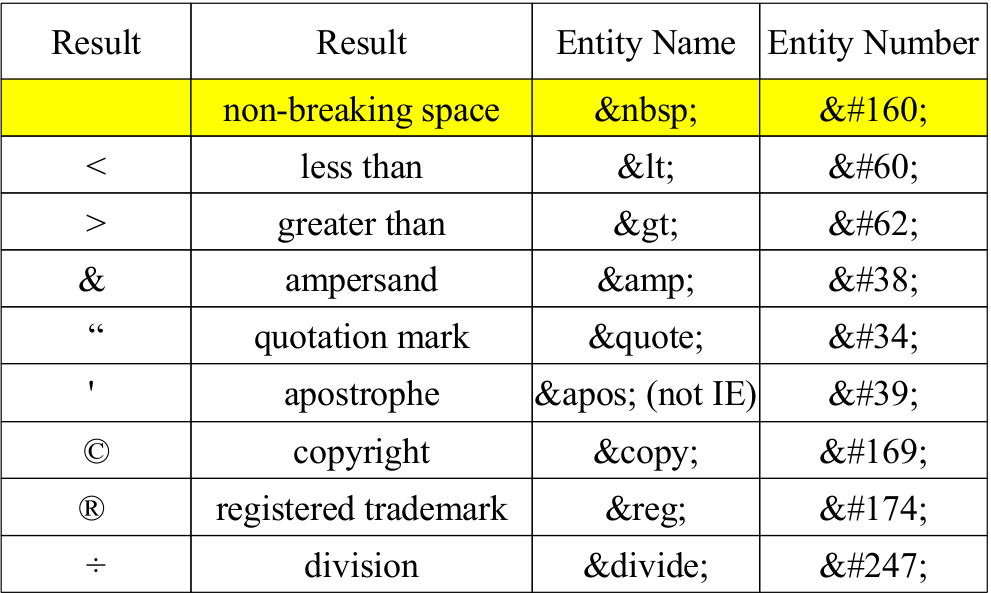
\includegraphics[scale=0.4]{hte}
\paragraph{Colors} Defined using hexadecimal notation for combination of RGB. \#FFFFFF $ = 255,255,255$. Pairs of two digits per color $(XX,XX,XX)\to(R,G,B)$
\begin{lstlisting}[language=html]
<tag color="red"> Hi </tag>
<tag color="#00FF00"> Hi </tag>
\end{lstlisting}
\subsection{CGI}Common Gateway Interface.
\paragraph{REST}REpresentational State Transfer. Server waits, packet arrives with request and info about caller. Server validates request, performs action if allowed. Returns answer to user with info about server. Forgets transaction and repeats.
\\stdin consists of inbound packet, stdout consists of outbound packet and the shell memory is the state information.
\paragraph{GET} Data is transferred inside query string. http://google.ca/search?q=test\&ie=utf-8
\\ Things after question mark indicate the data sent, parameters separated by \&. Allows for easy use of back buttons, easy to debug, but less secure than post(text shown in query, logged by server). Data is placed into shell memory.
\paragraph{Interfacing C and GET}
\begin{lstlisting}[language=c]
#include <stdlib.h>
char *data = getenv("QUERY_STRING"); //?thing=value&...
\end{lstlisting}
\paragraph{POST} Data transferred as part of query packet. More secure. Doesn't always work with back buttons. Harder to debug (need software to read). Data is placed into stdin.
\paragraph{Interfacing with C and POST}
\begin{lstlisting}[language=c]
#include <stdlib.h>
int n = atoi(getenv("CONTENT_LENGTH")); // Length of input
char string[n];
fgets(string,n+1,stdin);
\end{lstlisting}
\paragraph{Output to Browser}Must begin with:
\begin{lstlisting}[language=c]
printf("Content-Type: text/html\n\n");
printf("Content-Type: text/plain\n\n"); //Just the raw text, no html
\end{lstlisting}
If printing html, you then have to print the respective tags and all. Programs should be in the cgi-bin folder in public\_html (to work with our system). Bash scripts end in .sh, Python end in .py and compiled C programs end in .cgi
\section{Python}
Python is an interpreted language, not compiled. To run a Python script:
\begin{lstlisting}[language=bash]
python script.py
\end{lstlisting}
or, if you put the shabang at the top and make the script executable:
\begin{lstlisting}[language=bash]
./script.py
\end{lstlisting}
An interpreter takes the source code, interpretes it in someway to send it to the CPU. A compiler takes the source code and converts it into machine language, which it then sends to the CPU.
\\ There are no braces for functions and the like in Python, scope is defined by indentation.
\paragraph{Comments}~
\begin{lstlisting}[language=python]
# Comment
"""Multi-line comment
Line 2"""
\end{lstlisting}
\paragraph{Function}~
\begin{lstlisting}[language=python]
def funcname(params):
    """Stuff"""
    return 0
# Function is an object
funcname.__doc__ # Gives you comment "Stuff"
funcname.__name__ # Gives you funcname
\end{lstlisting}
Functions must be defined before use. There is no main function. To simulate a main:
\begin{lstlisting}[language=python]
if __name__=="main":
    do stuff
# or
def main():
    do stuff
main()
\end{lstlisting}
\paragraph{Importing}~
\begin{lstlisting}[language=python]
import FILE # Imports the whole file
from FILE import OBJECT # Only part of it
\end{lstlisting}
Some libraries to know:
\begin{lstlisting}[language=python]
import os
x = os.listdir("PATH")
if os.path.isfile("FILENAME")
if os.path.isdir("DIRNAME")

import cgi
form = cgi.FieldStorage()
if form.has_key('x'):
    thevalue = form["x"]

import urllib
urllib.quote(s) # "~e" -> "%7e"
urllib.unquote(s) # "%7e" -> "~e"
urllib.urlencode(dict) # dict -> query string
\end{lstlisting}
\paragraph{Conditionals and Loops}
\begin{lstlisting}[language=python]
if n>1 :
    do stuff
elif n=0:
    other thing
else :
    something else

if 0<n<9000 # Nice
if x <> y # x not in y
if not true
if true and false
if true or false

for x in y:
    do stuff

for i in range(x,y) # x to y-1
# You can leave out 2nd arg for range, will just do 0 to arg

while something:
    do stuff
\end{lstlisting}
No case statements, have to use if and elif.
\paragraph{Booleans}
\begin{itemize}
\item $0$ is false, all other numbers are true.
\item ``'' is false, all other strings true.
\item $[]$ false, all other lists true
\item () false, all other tuples true
  \item \{\} false, all other dictionaries true
\end{itemize}
\paragraph{Strings}
\begin{itemize}
\item Single quotes: literal, un-processed.
\item Double quotes: processed, can use \% operators like in C
  \item Triple quotes: multi-line Strings or ocmments
\item Can concatenate Strings with $+$ like in Java
\end{itemize}
\begin{lstlisting}[language=python]
# Note, Python 2.x print statements
print "%s me %s" %(x,y) # Vars x and y go in %s
\end{lstlisting}
Operations:
\begin{itemize}
\item Concatenation with $+$
\item Repetition with $*$
\item Indexing:
\begin{lstlisting}[language=python]
"abc"[1] # "b"
\end{lstlisting}
\item Slicing (substrings)
\begin{lstlisting}[language=python]
"abcdef"[0:2] # String from 0 to 2-1, "ab"
"abcdef"[1:] # String from 1 to end
\end{lstlisting}
\item len()
\item
\begin{lstlisting}[language=python]
"bc" in "abc" #True
"bc" not in "abc" #False
\end{lstlisting}
\item center, returns string surrounded by spaces to make it $n$ characters long.
\begin{lstlisting}[language=python]
a.center(n)
\end{lstlisting}
\item count, how many times item is in string
\begin{lstlisting}[language=python]
a.count("abc")
\end{lstlisting}
\item a.ljust(n), left justifies a in width n
\item a.rjust(n), right justifies
\item a.upper(), returns a in uppercase
\item a.lower(), lowercase
\item a.index(``abc'') returns index of first occurence of abc in a, error if not
\item a.find(``abc'') returns index of first occurence of abc in a, $-1$ if not found
\item a.replace(old,new) replaces all old by new
\end{itemize}
\paragraph{Types}
\begin{itemize}
\item Dictionary: like an array, but names instead of indicides. $\{idx1:val1,\ldots,idxn:valn\}$
  \\ To get the value of an index:
\begin{lstlisting}[language=python]
d = {"a":"b", "c":"d"}
d['a'] # Gives you b

d.keys() # Returns dict_keys obj
d.values() # Returns dict_values
d.items() # Returns tag+obj, dict_items
d.get("a") # Gives you b
d.get("f","a") # Gives val ass with f, a otherwise
"a" in d # key in d, true
"a" not in d # false

# Can auto add / replace stuff
d['a'] = "new"
d["e"] = "f"
del d['a']
d.clear()
\end{lstlisting}
\item List: $[val1,\ldots,valn]$
\begin{lstlisting}[language=python]
l = ["a","b","c","d"]
d[0] # "a"
d[-1] # "d", wraps around
d[1:3] # From 1 to 3, excluding 3
# ["a","b"]
# 2 methods of appending
d = d+["e"]
d+= ["e"]
x = [1,2]*3 # gives you list 3 times
# [1,2,1,2,1,2]
x.append(3)
x.insert(2,"a") # inserts a at position 2, shifts rest
x.extend([3,4]) # Same as append?
x.index(3)
x.remove(3)
x.pop()
x.push()
len(x) # Length of x
"3" in x # False since removed
\end{lstlisting}
\item Tuple: $(val1,\ldots,valn)$, a \textbf{constant} list.
  \\ Same indexing options as lists, with len function. Most other functions are not allowed (tuple can't be modified).
\end{itemize}
\paragraph{Declaring Variables} No syntax, just set var = value. 
\paragraph{Mapping}~
\begin{lstlisting}[language=python]
li = [1, 9, 8, 4]
li2 = [x*2 for x in li] # li2 = [2, 18, 16, 8]
\end{lstlisting}
\paragraph{Joining and Splitting}~
\begin{lstlisting}[language=python]
params = {"one":"1","two":"2"}
y=["%s=%s"%(k,v) for k,v in params.items()]
# y = ["one=1","two=2"]
w = ";".join(y)
# w = "one=1;two=2"
z = w.split(";")
# z = ["one=1","two=2"]
a = params.items();
# a = [(one,1), (two,2)]
\end{lstlisting}
\paragraph{Files}~
\begin{lstlisting}[language=python]
try:
    REF = open("file","type")#type=r,rb,w,wb,a,ab
except IOError:
    #deal with error
except:
    # catches all errors
else: 
    # No error
finally:
    # cleanup
\end{lstlisting}
Can have multiple excepts like catches in Java.
\begin{lstlisting}[language=python]
REF.mode # returns mode
REF.name # returns filename
REF.tell() # returns offset in bytes
REF.seek(BYTES,MODE) # 0=absolute, 1=relative, 2=eof relative
REF.read(BYTES)
REF.readline()
REF.readline(n) # Read first n chars of line
REF.readlines() # List with each cell being a line
REF.readlines(n) # n lines
REF.write("stuff")
REF.close()
REF.closed # Boolean
\end{lstlisting}
\paragraph{I/O}
Getting input from a user:
\begin{lstlisting}[language=python]
# Note raw_input() is input() in python 3.x
userInput = raw_input("This is printed and then waits until CR")
# or
import sys
sys.stdout.write("Give me input\n")
value = sys.stdin.readline()
\end{lstlisting}
\paragraph{Command Line Args}~
\begin{lstlisting}[language=python]
len(sys.argv)
print argv[1]+argv[2]
\end{lstlisting}
\paragraph{Casting}~
\begin{lstlisting}[language=python]
x = "53"
y = int(x)
z = y+3 # 56

ord('a') # char to int -> 97
chr(104) # int to char -> h
str(10) # int to str
\end{lstlisting}
\paragraph{Objects}Everything in Python is an object, even functions.
\\ Defining your own objects:
\begin{lstlisting}[language=python]
class NAME(PARENTLIST): # parentlist optional, comma sep, like extends
    def __init__(self, paramlist): #Constructor, self is like this
        self.thing = 5 # public
        self.__thing2 = 4 # private
\end{lstlisting}
Instantiating an object:
\begin{lstlisting}[language=python]
ref = NAME(paramlist) # no self
ref = none # Like null, python has garbage collector
\end{lstlisting}
\paragraph{Inheritance}
\begin{lstlisting}[language=python]
class InterestAccount(BankAccount):
    def deposit(self, amount):
        BankAccount.deposity(self,amount)
        self.balance = self.balance * 1.03
\end{lstlisting}
Inherits parents functions, can replace/modify them and add more.
\paragraph{Misc}
Complex numbers in python:
\begin{lstlisting}[language=python]
m = (2+4j) #j is imaginary part
\end{lstlisting}
Sets:
\begin{lstlisting}[language=python]
import sets
emptySet = sets.Set()
B = sets.Set([1,2,3])
C = sets.Set([3,4,5])
D = B.union(C)
E = B.intersection(C)
B.issuperset(C)
B.issubset(C)
\end{lstlisting}
\end{document}
%%% Local Variables:
%%% mode: latex
%%% TeX-master: t
%%% End:
